\section{Introduzione alle Reti Neurali}
\subsection{Il modello di McCulloch-Pitts}
Un modello pensato dai due tizi qui presenti,
\begin{itemize}
    \item Warren McCulloch
    \item Walter Pitts

\end{itemize}

Era formato da:
\begin{itemize}
    \item Un insieme di neuroni
    \item Un insieme di connessioni tra i neuroni
    \item Un insieme di pesi associati alle connessioni
    \item Una funzione di attivazione
    \item Una funzione di output
\end{itemize}

Quindi immaginiamo $x_1, x_2, \dots, x_n$ che vengono dati come input, e quello
che viene fuori è un valore di $y \in \{0,1\}$. Questo è un modello di
classificazione binaria.

In soldoni, in deep learning si usa un vettore di numeri per tirare fuori un
altro vettore di numeri.

Nella maggior parte del tempo, però, non lavoriamo solamente con i dati.
\begin{itemize}
    \item immagini
    \item Testo
    \item Audio
    \item \dots
\end{itemize}
Non ci sono concetti di foto, video, immagini. L'unico concetto che esiste
è quello dei numeri.

\subsection{Modello di Rosenblatt}
Qui il modello è leggermente diverso. Gli elementi in questo modello sono i
seguenti:
\begin{itemize}
    \item Valori di input: $x_i$
    \item Funzione di attivazione: $\phi$
    \item Pesi degli archi: $w_i$
    \item Bias: $b$
\end{itemize}

\begin{equation}
    h(x|w,b) = h(\sum_{i=1}^l w_i\cdot x_i -b) = h(\sum_{i=1}^l w_i\cdot x_i) = \textit{sign}(w^Tx)
\end{equation}

\textbf{Nota:} Quando il \textbf{bias} non viene specificato, allora
si assume che sia 0.

I pesi $w_i$ sono collegati archi che vanno da $x_i$ al prossimo neurone. Sia
il valore di input che il peso sono \textbf{numeri reali}. Non sono lo stesso
valore, hanno solamente il formato di \textit{reale} che è uguale tra loro. Ciò
che viene fatto è solamente la somma della prodotto tra ogni peso $w_i$ e $x_i$
\textbf{meno} il bias.

\textbf{La funzione di attivazione:} Dipende. Ogni funzione che ha \textit{2 stati} va bene per noi. Una funzione di attivazione può essere una qualsiasi che in un
punto ha valore 1 e in un altro ha valore -1.

\subsection{Esempio con 2 neuroni}.

Immaginiamo di avere un piano cartesiano con una retta che interseca in 2
punti.

\begin{equation}
    sign(w_1\cdot x_1 + w_2\cdot x_2)
\end{equation}

Il parametro della funzione non è altro che \textbf{l'equazione di una retta.}

In particolare, se consideriamo la reta che separa gli spazi del piano, vediamo
che la retta è \textbf{capace di separare 2 punti nel piano.}

\textbf{Cosa abbiamo}:
\begin{itemize}
    \item Un neurone
    \item 2 valori in input
    \item 2 pesi
\end{itemize}

Con la funzione di attivazione \textbf{sign} si avrà come output una retta che
separa dei punti.
\begin{tikzpicture}[scale=1.5]
    % Asse x
    \draw[->] (-2,0) -- (2,0) node[right] {$x$};
    % Asse y
    \draw[->] (0,-2) -- (0,2) node[above] {$y$};

    % Punto A
    \coordinate (A) at (-1.5,1);
    \fill[red] (A) circle (2pt) node[above left] {$A$};

    % Punto B
    \coordinate (B) at (1,0.5);
    \fill (B) circle (2pt) node[above right] {$B$};

    % Retta
    \draw[dashed] (-2,-0.25) -- (2,1.75) node[right] {$r$};
\end{tikzpicture}

\textbf{Nota}: Quando è utile avere un valore output che non è una separazione di punti in un piano? Nel caso della \textbf{regressione}.

\textbf{Oltre la funzione sign}:
\begin{itemize}
    \item Funzione di attivazione lineare
    \item Funzione di attivazione sigmoid
    \item Funzione di attivazione Tanh
\end{itemize}

\subsection{Rappresentazione le funzioni logiche}:

\subsubsection{AND}
Immaginiamo di avere:
\begin{itemize}
    \item $x_1,x_2 \in \{0,1\}$
    \item Bias= -30
    \item Funzione di attivazione: Logistica o Sigmoid
\end{itemize}

Come facciamo a rappresentare un AND?

\begin{equation}
    h(x)= g(-30+20x_1 +20x_2)
\end{equation}
\begin{center}
    \begin{tabular}{|c|c|c|}
        \hline
        $x_1$ & $x_2$ & $h(x)$ \\
        \hline
        0     & 0     & 1      \\
        0     & 1     & 0      \\
        1     & 0     & 0      \\
        1     & 1     & 1      \\
        \hline
    \end{tabular}
\end{center}

Lo stesso ragionamento vale per:
\begin{itemize}
    \item OR
    \item NOT
    \item (NOT $x_1$) AND (NOT $x_2$)
\end{itemize}

\subsubsection{Il problema dello XOR}
\begin{quote}
    Il percettrone non può imparare regioni che non sono linearmente separabili.
\end{quote}

\begin{figure}[H]
    \begin{center}
        \begin{tikzpicture}[scale=1.5][h!]
            % Asse x
            \draw[->] (-2,0) -- (2,0) node[right] {$x$};
            % Asse y
            \draw[->] (0,-2) -- (0,2) node[above] {$y$};

            % Punto A
            \coordinate (A) at (0,1);
            \fill[red] (A) circle (2pt) node[above left] {$A$};

            % Punto B
            \coordinate (B) at (0,0);
            \fill (B) circle (2pt) node[above right] {$B$};

            \coordinate (B) at (1,0);
            \fill (B)[red] circle (2pt) node[above right] {$B$};

            \coordinate (B) at (1,1);
            \fill (B) circle (2pt) node[above right] {$B$};
        \end{tikzpicture}
        \caption{XOR non possibile con 1 percettrone}
    \end{center}

\end{figure}

Come vediamo qui non possoamo tracciare una retta per dividere i due punti. In
questo caso ci serve una funzione \textbf{non lineare}.

La soluzione a questo problema è \textbf{aggiungere LAYER} alla rete neurale.
Aggiungere un layer significa aggiungere un neurone successivamente ad un
altro.

Maggiore è il numero di layer, maggiore diventa la potenza espressiva della
rete. Praticamente possiamo catturare qualsiasi cosa aggiungendo layer alla
rete. Questo è \textbf{il vero potere del deep learning}.

\usetikzlibrary{positioning}
\begin{figure}[H]
    \begin{center}

        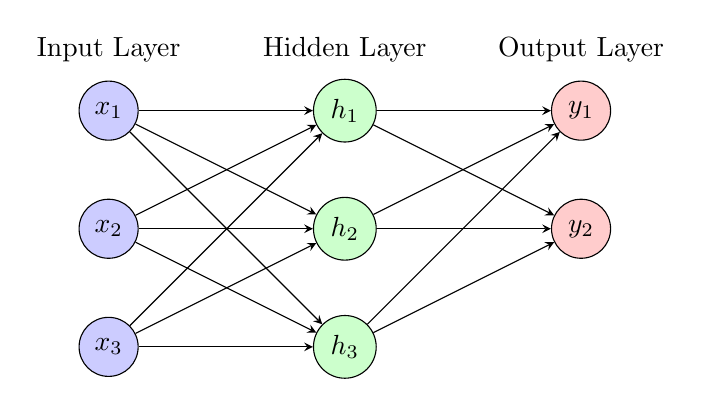
\begin{tikzpicture}[x=1.5cm, y=1.5cm, >=stealth]

            % Input Layer
            \foreach \i in {1,2,3}
            \node[circle, draw, fill=blue!20, minimum size=0.75cm] (I\i) at (0,-\i) {$x_{\i}$};

            % Hidden Layer
            \foreach \i in {1,2,3}
            \node[circle, draw, fill=green!20, minimum size=0.75cm] (H\i) at (2,-\i) {$h_{\i}$};

            % Output Layer
            \foreach \i in {1,2}
            \node[circle, draw, fill=red!20, minimum size=0.75cm] (O\i) at (4,-\i) {$y_{\i}$};

            % Connect Layers
            \foreach \i in {1,2,3}
            \foreach \j in {1,2,3}
            \draw[->] (I\i) -- (H\j);

            \foreach \i in {1,2,3}
            \foreach \j in {1,2}
            \draw[->] (H\i) -- (O\j);

            % Labels
            \node[above=0.5cm] at (I1) {Input Layer};
            \node[above=0.5cm] at (H1) {Hidden Layer};
            \node[above=0.5cm] at (O1) {Output Layer};

        \end{tikzpicture}
    \end{center}
    \caption{Neural Network con 1 hidden layer}
\end{figure}

\subsection{Gli ingredienti di una rete neurale}
\subsubsection{Il grafo g}
Un grafo $g = \{N,E\}$ è un grafo diretto pesato con label.

Ogni nodo $i \in N$ viene chiamato \textbf{neurone} o \textbf{percettrone}. Per
ogni nodo ci sono 2 targhette:
\begin{itemize}
    \item Un valore $a_i$ che viene chiamato \textbf{attivazione}
    \item Una funzione di attivazione $f_i$ che viene applicata all'attivazione, che
          produce un output $z_i$
\end{itemize}

Ogni arco $e = \{j \in N \rightarrow i \in N\} \in E$ associato con un peso
$w_{j,i}$.

Ogni nodo $i$ è anche coinvolto con un arco speciale, con un nodo fantasma, che
viene chiamato \textbf{bias} $b_i$.

\textbf{Nota:} $z_i = f_i(a_i)$. E $a_i = b_i  + \sum_{j:j\rightarrow i \in E} w_{j,i}z_j$

La combinazione dei neuroni connessi costruisce il grafo. I nodi che
condividono gli stessi input sono raggruppati in \textbf{layers}.

\usetikzlibrary{positioning}
\begin{figure}[H]
    \begin{center}

        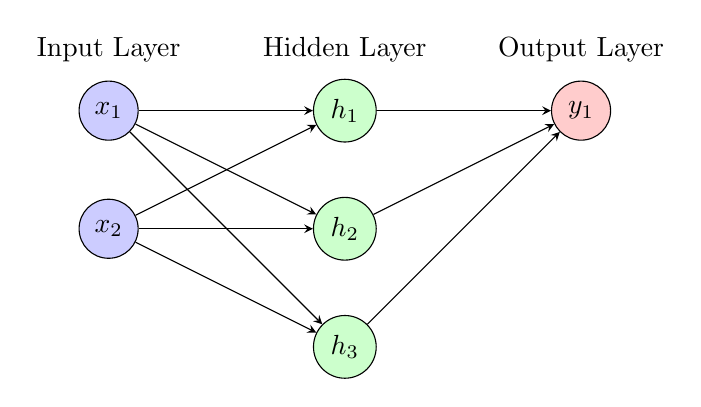
\begin{tikzpicture}[x=1.5cm, y=1.5cm, >=stealth]

            % Input Layer
            \foreach \i in {1,2}
            \node[circle, draw, fill=blue!20, minimum size=0.75cm] (I\i) at (0,-\i) {$x_{\i}$};

            % Hidden Layer
            \foreach \i in {1,2,3}
            \node[circle, draw, fill=green!20, minimum size=0.75cm] (H\i) at (2,-\i) {$h_{\i}$};

            % Output Layer
            \foreach \i in {1}
            \node[circle, draw, fill=red!20, minimum size=0.75cm] (O\i) at (4,-\i) {$y_{\i}$};

            % Connect Layers
            \foreach \i in {1,2}
            \foreach \j in {1,2,3}
            \draw[->] (I\i) -- (H\j);

            \foreach \i in {1,2,3}
            \foreach \j in {1}
            \draw[->] (H\i) -- (O\j);

            % Labels
            \node[above=0.5cm] at (I1) {Input Layer};
            \node[above=0.5cm] at (H1) {Hidden Layer};
            \node[above=0.5cm] at (O1) {Output Layer};

        \end{tikzpicture}
    \end{center}
    \caption{Neural Network con 1 hidden layer}
\end{figure}

Il risultato finale dipende da tutti i parametri del grafo, e anche dal tipo di
funzione di attivazione che viene usata.
\begin{quote}
    Ma come facciamo a scegliere il corretto valore dei parametri del grafo?
\end{quote}

\subsubsection{La funzione di loss}
Il grafo è un operatore algebrico non lineare: $g(\vec{x}|W,B)$. In questo
grafo non sappiamo il valore di \textbf{B e W}. La fase di apprendimenti di una
rete consiste nel trovare il \textbf{migliore} valore per W e per B. Ma cosa
intendiamo con \textbf{migliore?}.

Formalmente, l'unico modo che abbiamo per definire la conezione di migliore, è
quello di \textit{approssimare al meglio la funzione che vogliamo trovare}.

%scrivi un vettore verticale di x_1 a x_m e un vettore verticale di y_1 a y_m%

Consideriamo il valore di una funzione $F$ su $x_i$ e il vero valore di $y_i$.
Noi vogliamo minimizzare la differenza tra $F(x_i)$ e $y_i$.

\begin{equation}
    \min_{W,B}\frac{1}{n} \sum_{i=1}^n loss(\vec{y_i}, g(x_i|W,B))
\end{equation}
con:
\begin{itemize}
    \item $loss(\vec{y_i}, g(x_i|W,B))$ è una funzione che misura la differenza tra $y_i$ e $g(x_i|W,B)$
    \item $n$ è il numero di esempi
    \item $W$ e $B$ sono i parametri del grafo
    \item $g(x_i|W,B)$ è il valore di output del grafo
    \item $\vec{y_i}$ è il valore di output vero
\end{itemize}

La funzione di \textbf{loss} dipende dal tipo di task che dobbiamo svolgere.

\subsubsection{Funzione di loss per Regressione}
\textbf{Mean Absolute Error}:
\begin{equation}
    \frac{1}{n} \sum_{i=1}^n |y_i - g(\vec{x_i}|W,B)|
\end{equation}
\begin{itemize}
    \item Considera tutti gli errori con lo stesso peso
    \item \textbf{Non è differenziabile in 0}
\end{itemize}

\textbf{Mean Squared Error}:
\begin{equation}
    \frac{1}{n} \sum_{i=1}^n (y_i - g(\vec{x_i}|W,B))^2
\end{equation}

\begin{itemize}
    \item Gli errori più grandi hanno un peso maggiore
    \item \textbf{È differenziabile in 0}
    \item \textbf{È più sensibile agli outliers}
\end{itemize}

\textbf{Domanda:} quale si usa tra le due? Dall'approccio greedy, \textbf{usa entrambe}.

\textbf{Esistono anche altre funzioni:}
\begin{itemize}
    \item Smooth Absolute Error
    \item Huber Loss
\end{itemize}

\subsubsection{Funzione di loss per classificazione}

\textbf{Binary Cross Entropy [BCE]}
Viene usata se $y_i \in \{0,1\}, g(\vec{x}|W,B) \in [0,1]$.
\begin{equation}
    BCE = -\frac{1}{n} \sum_{i=1}^n y_i \log(g(\vec{x_i}|W,B)) - (1-y_i)\log(1-g(\vec{x_i}|W,B))
\end{equation}

\textbf{Categorical Cross Entropy [CCE]}
\begin{equation}
    CCE = -\frac{1}{n} \sum_{i=1}^n \sum_{j=1}^m y_{i,j} \log(g(\vec{x_i}|W,B))_j
\end{equation}
\subsection{L'ottimizzatore o}
Come risolviamo il problema di:
\begin{equation}
    \min_{W,B} \frac{1}{n} \sum_{i=1}^n loss(\vec{y_i}, g(\vec{x_i}|W,B))
\end{equation}

Il problema lo risolviamo calcolando il \textbf{gradiante} della funzione loss,
lo poniamo uugale a 0 e controlliamo se siamo in un punto di \textbf{massimo,
    minimo o punto di sella}.

\begin{equation}
    \frac{\partial loss}{\partial W} = 0
\end{equation}

Abbiamo bisogno di un metodo iterativo per trovare una soluzione. Ci vuole
un'\textbf{euristica}. Tipicamente, siamo soddisfatti di un \textbf{minimo
    locale}, e si utilizza, appunto, il \textbf{metodo di discesa del gradiente}.

\textbf{Differenza minimo locale e globale}

\begin{figure}[H]
    \begin{center}

        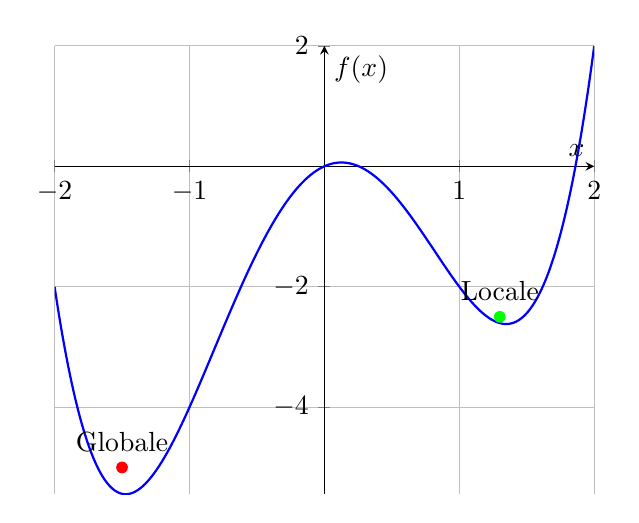
\begin{tikzpicture}
            \begin{axis}[
                    xlabel=$x$,
                    ylabel=$f(x)$,
                    domain=-2:2,
                    samples=400,
                    axis lines=middle,
                    grid
                ]
                \addplot[blue,thick]{x^4 - 4*x^2 + x};
                \node[red,circle,fill,inner sep=1.5pt,label={90:Globale}] at (axis cs:  -1.5,-5) {};
                \node[green,circle,fill,inner sep=1.5pt,label={90: Locale}] at (axis cs:1.3,-2.5) {};
            \end{axis}
        \end{tikzpicture}
        \caption{Differenza tra minimo locale e globale}
    \end{center}

\end{figure}

\subsubsection{Il metodo di discesa del gradiente}
Sia $F(\vec{x})$ una funzione differenziabile.
\begin{itemize}
    \item $F(\vec{x})$ decresce più veloce nella direzione del gradiente negativo
    \item $F(\vec{x})$ cresce più veloce nella direzione opposta al gradiente
\end{itemize}

\begin{equation}
    a^{new} = a^{old} - \eta \cdot \nabla F(a^{old})
\end{equation}

Il parametro $\eta$ viene chiamato \textbf{learning rate} e determina il
comportamento del'ottimizzazione. Da notare che e' l'unico \textbf{parametro}.
\begin{figure}[H]
    \begin{center}

        \begin{tikzpicture}[]
            \begin{axis}[
                    xlabel=$x$,
                    ylabel=$f(x)$,
                    domain=-2:2,
                    samples=200,
                    axis lines=middle,
                    width=10cm,
                    height=6cm,
                    xmin=-2,
                    xmax=2,
                    ymin=-4,
                    ymax=5,
                    xtick={-1, 0, 1},
                    xticklabels={$-1$, $0$, $1$},
                    ytick={1, 3},
                    yticklabels={$f_{\text{min}}$, $f_{\text{max}}$},
                ]

                \addplot[blue,thick,domain=-1.5:1.5] {x^4 - 2*x^3 - 2*x^2 + 3*x + 1};

                % Frecce verso il minimo
                \draw[->, red, thick] (axis cs:-1.5,4) -- (axis cs:-1.3,3);
                \draw[->, red, thick] (axis cs:-1.3,3) -- (axis cs:-1.2,1.8);
                \draw[->, red, thick] (axis cs:-1.2,2) -- (axis cs:-1.1,1.1);
            \end{axis}
        \end{tikzpicture}
    \end{center}
    \caption{Discesa del gradiente}
\end{figure}

\textbf{Ci sono ancora problemi:} Questo metodo non è esente da problemi, quindi abbiamo:
\begin{itemize}
    \item Dipendentemente dal punto di inizio, abbiamo un risultato diverso. Dobbiamo
          capire che, giustamente, se ci accontentiamo di un minimo locale, non avremo
          quasi mai lo stesso minimo per ogni allenamento della rete.
\end{itemize}

\textbf{Nota:} con \textbf{topologia} intendiamo il numero di layer e il numero
di neuroni per layer.

Diciamo che in generale, gli steps per allenare una rete sono:
\lstset{mathescape}
\begin{lstlisting}
    for each topology T in $C_t$
        for each $\eta$ in $C_\eta$
            for each initialization I in $C_I$
                Applica la discesa del gradiente
\end{lstlisting}

\subsubsection{Il metodo di discesa del gradiente stocastico}
La differenza del metodo di discesa del gradiente stocastico è che, invece di
calcolare il gradiente su tutti i dati, si calcola il gradiente su un
sottoinsieme di dati.

Ciò che viene fatto, per ogni step, invece di prendere la derivata di ogni loss
function e poi fare i calcoli, prendo \textbf{un sample del mio dataset},
tipicamente chiamato \textbf{batch}. Ogni volta che calcolo la discesa del
gradiente, calcolo la derivata \textbf{NON PER TUTTO IL DATASET}, ma solamente
del \textbf{batch}. Questo OVVIAMENTE non mi assicura che ottimizzare ogni
batch mi ottimizza anche l'intero dataset, ma non c'è modo di lavorare
sull'intero dasaset, poiché questo è troppo grande e richiede troppo tempo.

Nonostante tutto, utilizzando questa tecnica \textbf{si ottengono risultati
    comunque accettabili}.

Il \textit{workflow} allora cambia in: \lstset{mathescape}
\begin{lstlisting}
    for each topology T in $C_t$
        for each $\eta$ in $C_\eta$
          for each initialization I in $C_I$
           for each batch size $b \in C_b$
             Applica la discesa del gradiente stocastica
\end{lstlisting}

\subsubsection{Linee guida sul learning rate}

\textbf{Epoca}: Un'epoca è un passaggio dell'approssimazione della funzione
\begin{figure}[H]
    \begin{center}

        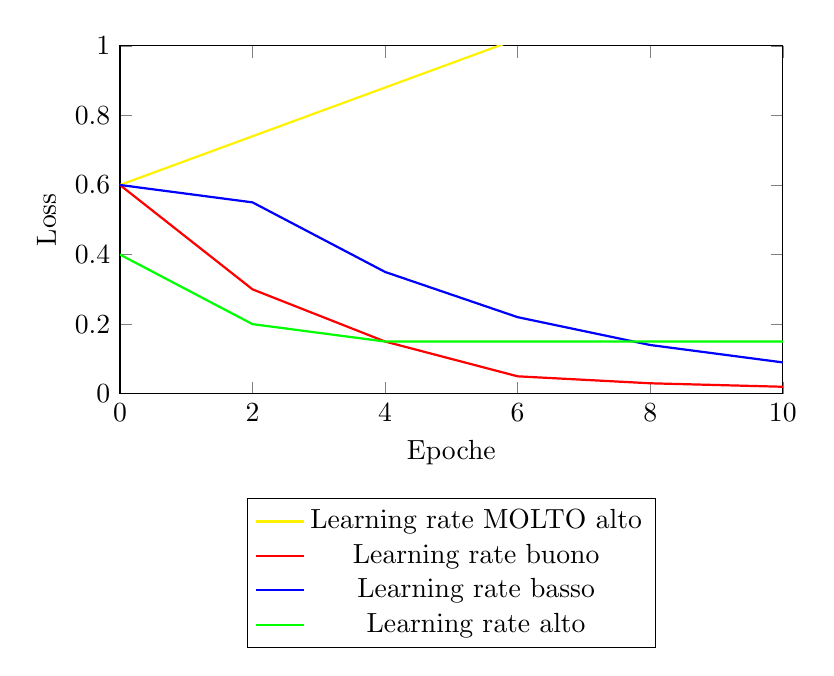
\begin{tikzpicture}
            \begin{axis}[
                    xlabel=Epoche,
                    ylabel=Loss,
                    width=10cm,
                    height=6cm,
                    xmin=0,
                    xmax=10,
                    ymin=0,
                    ymax=1,
                    xtick={0, 2, 4, 6, 8, 10},
                    ytick={0, 0.2, 0.4, 0.6, 0.8, 1},
                    legend style={at={(0.5,-0.3)},anchor=north},
                    legend entries={Learning rate MOLTO alto, Learning rate buono, Learning rate basso, Learning rate alto},
                ]

                \addplot[thick, yellow] coordinates {(0, 0.6) (10, 1.3)};
                \addplot[thick, red] coordinates {(0, 0.6) (2, 0.3) (4, 0.15) (6, 0.05) (8, 0.03) (10, 0.02)};
                \addplot[thick, blue] coordinates {(0, 0.6) (2, 0.55) (4, 0.35) (6, 0.22) (8, 0.14) (10, 0.09)};
                \addplot[thick, green] coordinates {(0, 0.4) (2, 0.2) (4, 0.15) (6, 0.15) (8, 0.15) (10, 0.15)};
            \end{axis}
        \end{tikzpicture}
    \end{center}
    \caption{Esempio di andamento della funzione di loss in base al learning rate}
\end{figure}

Analisi dei learning rate:
\begin{itemize}
    \item learning rate basso: troppo lento!
    \item learning rate alto: fermo con un minimo locale immediatamente
    \item learning rate MOLTO alto: non converge mai
    \item learning rate buono: decresce sempre e eventualmente converge
\end{itemize}

\textbf{Nota:} Il learning rate è un parametro che va \textbf{tunato}.
\begin{itemize}
    \item Se il learning rate è troppo alto, non si riesce a convergere poiché si salta
          il minimo
    \item Se il learning rate è troppo basso, si rischia di non convergere mai
\end{itemize}

Il nostro obiettivo è quello di avere un learning rate che sia \textbf{giusto}
e che permetta di avere un andamento della funzione di loss come quello in
rosso, cioé avere una buona diminuizione della loss andando avanti con le
epoche. Sempre decrescente e con la distanza minore dall'asse delle x.

\textbf{Domanda:} Vogliamo sempre la loss uguale a 0? \textbf{No.}
Perché? Perché a differenza che in statistica dove vogliamo avere un errore il minimo.
In deep learning non è così. Se la loss è 0, allora vuol dire che la rete ha
imparato a memoria i dati, e non è quello che vogliamo. Vogliamo che la rete
sia capace di generalizzare.

In particolare, noi \textbf{vogliamo fare predizioni}, sopratutto su
\textbf{istanze ancora non viste.} Se avessimo una loss uguale a 0,
probabilmente non saremmo in grado di avere delle predizioni decenti, poiché la
rete non è in grado di generalizzare. Avendo la loss non a 0 rendiamo la rete
capace di poter introdurre istanze ancora non viste in futuro.

Quindi, per statistica \textbf{loss = 0 : nice}, per \textbf{deep learning:
    insomma}.
